\documentclass[12pt]{article}
\usepackage{graphicx} 
\usepackage{amsmath}
\usepackage{amsthm}
\usepackage{graphicx}
\usepackage{enumerate}
\usepackage{natbib}
\usepackage{booktabs}
\usepackage{hyperref}
\hypersetup{colorlinks = true, linkcolor = blue, citecolor=blue, urlcolor = blue}
\usepackage{enumitem}
\newcommand{\blind}{0}
\addtolength{\oddsidemargin}{-.5in}%
\addtolength{\evensidemargin}{-.5in}%
\addtolength{\textwidth}{1in}%
\addtolength{\textheight}{1.3in}%
\addtolength{\topmargin}{-.8in}%
\usepackage{float}
\usepackage{array} 



\begin{document}



\def\spacingset#1{\renewcommand{\baselinestretch}%
{#1}\small\normalsize} \spacingset{1}


%%%%%%%%%%%%%%%%%%%%%%%%%%%%%%%%%%%%%%%%%%%%%%%%%%%%%%%%%%%%%%%%%%%%%%%%%%%%%%

\if0\blind
{
  \title{\bf The usage of bootstrap method in shape-restricted regression}
  \author{Guanghong Yi\\
  Jun Yan\\[1ex]
  Department of Statistics, University of Connecticut\\
}
  \maketitle
} \fi

\if1\blind
{
  \bigskip
  \bigskip
  \bigskip
  \begin{center}
    {\LARGE\bf The usage of bootstrap method in shape-restricted regression}
\end{center}
  \medskip
} \fi

\bigskip
\begin{abstract}
The bootstrap method is an important resampling technique used to estimate statistics on a population by repeatedly sampling the data. It is also an effective approach for estimating the measure of dispersion in a dataset, especially in regression analysis. However, in some cases, regression models need to be constrained with known characteristics such as monotonicity or curvature, for example, in growth curves, where the coefficients are forced to be non-negative. In such situations, spline regression is used for modeling. It is not always certain whether the bootstrap method can be directly applied to estimate the dispersion under these shape-restricted scenarios, especially for pointwise confidence intervals. In this article, we will demonstrate the usage of the bootstrap method in shape-restricted regression and proof the effectiveness of bootstrap for constructing pointwise confidence intervals in shape-restricted regression empirically.
\end{abstract}

\noindent%
{\it Keywords:}  bootstrap; shape-restricted regression; pointwise confidence interval; growth curve; splines regression
\vfill

\newpage
\spacingset{1.45} 
\section{Introduction}
\label{sec:intro}

Bootstrap is a powerful and important resampling method for estimating population parameters or assessing the accuracy of a statistical procedure by repeatedly sampling the data with replacement. Its effectiveness have been widely recognized in regression analysis. By bootstrap, we can estimate the standard errors of the regression coefficients. Even for unknown underlying population distributions, bootstrap method can resample the data with replacement and computes the regression coefficients for each resampled dataset. By repeating this process many times, it provides an empirical estimate of the standard errors, which can be valuable when the assumptions of traditional standard error estimation techniques are violated. It can also be used to construct confidence intervals for regression coefficients. By resampling the dataset, bootstrap can determining the percentile intervals of these coefficients, we can obtain approximate confidence intervals for the regression parameters. Bootstrap can also construct the approximate confidence interval for certain time points f(t)s in the function by simulating f'(t) certain times in certain time points. However, when dealing with shape-restricted regressions, where the coefficients are forced to adhere to specific constraints such as monotonicity or curvature, the effectiveness of bootstrap is not proved to be guaranteed. In this paper, we will demonstrate the usage of the bootstrap method in shape-restricted regression and proof the effectiveness of bootstrap for constructing pointwise confidence intervals in shape-restricted regression empirically.

The rest of the paper is organized as the follows. Section~\ref{Bootstrap Method for Constructing Confidence Intervals} gives a review of bootstrap method for constructing confidence intervals. Section~\ref{Shape Restricted Example} gives out a shape-restricted regression example and the usage of bootstrap to build the pointwise confidence intervals for certain time points. Section~\ref{Simulation Study} shows a simulation study to assess the performance of the methods.
explores the case where a combination of the first two scenarios occurs. An  
adjusted bootstrap procedure is proposed as a working solution in this case.  
Section~\ref{Conclusion} concludes with a discussion.




\section{Bootstrap Method for Constructing Confidence Intervals}
\label{Bootstrap Method for Constructing Confidence Intervals}

The bootstrap method is a powerful resampling technique used to construct confidence intervals for population parameters or estimates when the underlying distribution is unknown or difficult to determine. It is useful in regression analysis to estimate the uncertainty associated with the regression coefficients or for certain time points inside the regression function. Specifically, the bootstrap method basically contains three steps:

\begin{enumerate}[label=\arabic*.]
    \item Let \(v\) represent a population parameter of interest (e.g., mean, median, standard deviation, etc.), which is drawn from an unknown population distribution \(F\).
    \item Generate a bootstrap sample \(x_1, x_2, \ldots, x_n\) from the population, and they are referred to as the original sample dataset.
    \item Let \(u\) represent a statistic calculated from the bootstrap original sample dataset.
    \item Using the data in the original sample dataset as the "population," perform nonparametric resampling with replacement to obtain a resampled sample (also known as the Bootstrap sample), denoted as \(x_1^*, x_2^*, \ldots, x_n^*\) (the number of data points in the Bootstrap sample must be the same as the number of data points in the original sample).
    \item Let \(u^*\) represent the statistic computed by the Bootstrap sample datasets, and this will be the bootstrap estimated statistic for the population statistic.

\end{enumerate}

Bootstrap method has been proved that it is an excellent method to estimate statistic, the \(u^*\) we obtained from the resampling dataset is a good estimator for the \(v\) as a population parameter. According to the bootstrap method, we can also calculate the confidence interval for the parameters, or the coefficients of a certain regression, or for certain time points in the regression.



Should I give out an example for a normal regression and calculate its pointwise confidence interval by certain time points?

It has been proved that the bootstrap method can be used as a good estimator for the pointwise confidence interval in linear regressions and non-linear regressions, but in certain special cases(i.e. shape-restricted splines regressions) we have not prove that it is a good method to build pointwise confidence interval via bootstrap.

Shape-restricted splines regressions are piecewise polynominal, differentiable to a certain degree and have certain restrictions like monotonicity or convexity. Given these conditions, the application of the bootstrap method to estimate pointwise confidence intervals for specific time points within the regression cannot be guaranteed to be suitable. And in the article we gives out an example of shape-restricted regression and the method to fit confidence interval for certain time points in the function.









\section{Shape Restricted Example}
\label{Shape Restricted Example}

In some situations the regression is forced to be shape-restricted to improve the predictive performance and reduce overfitting if the underlying regression function takes the specific form. The example is given from R package SemiPar. And we fit the shape-restricted regression by the R package Splines2 based on the article \cite{wang2021shape}. Splines2 provides implementation of those spline basis functions via R language, and we use that to build a non-decreasing curve by i-spline that force the coefficients to be non-negative with degree of freedom = 6.

Then, we selected 10 time points, denoted as $f(t)$, with equal intervals from the dataset. We performed bootstrap resampling 1000 times to obtain the 95\% quantile pointwise confidence interval for each points.

\begin{figure}[H]
  \centering
  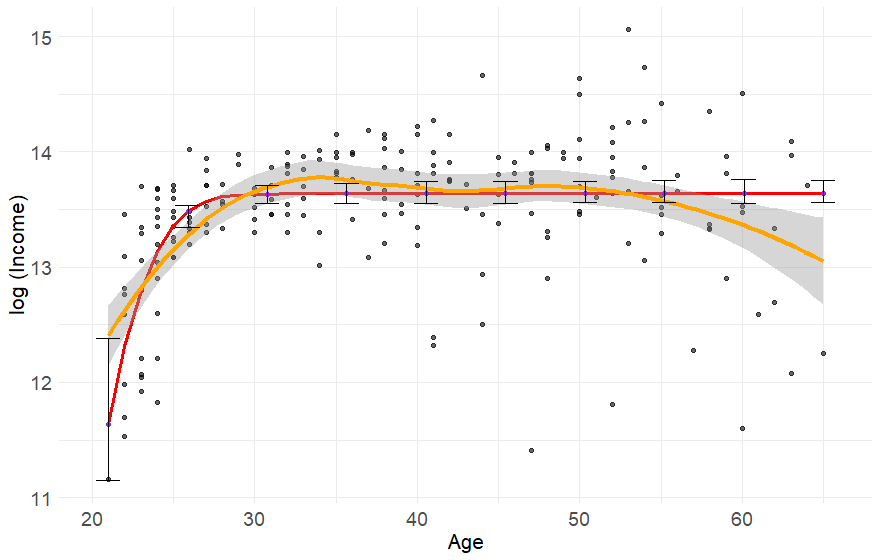
\includegraphics[width=0.8\textwidth]{SemiparCI.png}
  \caption{CI build for the shape-restricted regression}
  \label{fig:semipar}
\end{figure}











\section{Simulation Study}
\label{Simulation Study}

Since the underlying distribution is unknown, we need to perform a simulation study to test whether the fitted pointwise confidence interval is accurate for the regression.

We define three functions: \(y = 0.25(x - 0.9)\) , \(y = 0.02(x^3+1.2)\) , and \( y = 0.1 (5pnorm((x - 2) / 0.3) + 1)\) , and randomly generate 1000 points \(x\) and its corresponding values \(y\) with added noise. The noise is added from a standard normal distribution with \(\mu = 0\) and standard deviation \(1\). Let the paired values \((x, y\text{ with noise})\) be the dataset, and then we know the true values of \(y\) as well.

We fit shape-restricted i-splines regressions using degrees of freedom 6 to the dataset. We select 1, 5, 10, 15, 20, 25, 30 as the time points from the dataset and perform bootstrap resampling B = 1000 times to estimate the \(95\%\) quantile pointwise confidence intervals for each of the selected time points. We repeat this process 1000 times to see how many times these confidence intervals can contain the true result. The results are shown below:



\begin{table}[ht]
  \centering
  \caption{Results of function \(y = 0.25(x - 0.9)\) for different degrees of freedom}
  \begin{tabular}{|c|c|c|c|c|}
    \hline
    \textbf{x} & \textbf{y} & \textbf{df\_6} & \textbf{df\_10} & \textbf{df\_15} \\
    \hline
    \multicolumn{5}{|c|}{B = 1000} \\
    \hline
    1 & 0.025 & 0.936 & 0.944 & 0.939 \\
    \hline
    5 & 1.025 & 0.960 & 0.958 & 0.948 \\
    \hline
    10 & 2.275 & 0.956 & 0.950 & 0.951 \\
    \hline
    15 & 3.525 & 0.959 & 0.954 & 0.954 \\
    \hline
    20 & 4.775 & 0.941 & 0.949 & 0.961 \\
    \hline
    25 & 6.025 & 0.953 & 0.946 & 0.942 \\
    \hline
    30 & 7.275 & 0.919 & 0.955 & 0.947 \\
    \hline
    \multicolumn{5}{|c|}{B = 2000} \\
    \hline
    1 & 0.025 & 0.936 & 0.944 & 0.939 \\
    \hline
    5 & 1.025 & 0.960 & 0.958 & 0.948 \\
    \hline
    10 & 2.275 & 0.956 & 0.950 & 0.951 \\
    \hline
    15 & 3.525 & 0.959 & 0.954 & 0.954 \\
    \hline
    20 & 4.775 & 0.941 & 0.949 & 0.961 \\
    \hline
    25 & 6.025 & 0.953 & 0.946 & 0.942 \\
    \hline
    30 & 7.275 & 0.919 & 0.955 & 0.947 \\
    \hline
  \end{tabular}
\end{table}



\begin{table}[ht]
  \centering
  \caption{Result of function  \(y = 0.02(x^3+1.2)\)}
\begin{tabular}{|c|c|c|c|c|}
    \hline
\textbf{x} & \textbf{y} & \textbf{df\_6} & \textbf{df\_10} & \textbf{df\_15} \\
    \hline
    1 & 0.025 & 0.893 & 0.940 & 0.959 \\
    \hline
    5 & 1.025 & 0.932 & 0.948 & 0.958 \\
    \hline
    10 & 2.275 & 0.937 & 0.948 & 0.941 \\
    \hline
    15 & 3.525 & 0.942 & 0.951 & 0.953 \\
    \hline
    20 & 4.775 & 0.939 & 0.951 & 0.957 \\
    \hline
    25 & 6.025 & 0.952 & 0.959 & 0.963 \\
    \hline
    30 & 7.275 & 0.947 & 0.943 & 0.943 \\
    \hline
  \end{tabular}
\end{table}


\begin{table}[ht]
  \centering
  \caption{Result of function \( y = 0.1 (5pnorm((x - 2) / 0.3) + 1)\) when B = 1000}
\begin{tabular}{|c|c|c|c|c|}
    \hline
\textbf{x} & \textbf{y} & \textbf{df\_6} & \textbf{df\_10} & \textbf{df\_15} \\
    \hline
    1 & 0.025 & 0.686 & 0.847 & 0.901 \\
    \hline
    5 & 1.025 & 0.279 & 0.800 & 0.852 \\
    \hline
    10 & 2.275 & 0.947 & 0.937 & 0.942 \\
    \hline
    15 & 3.525 & 0.937 & 0.953 & 0.961 \\
    \hline
    20 & 4.775 & 0.929 & 0.950 & 0.957 \\
    \hline
    25 & 6.025 & 0.953 & 0.924 & 0.922 \\
    \hline
    30 & 7.275 & 0.919 & 0.858 & 0.832 \\
    \hline
  \end{tabular}
\end{table}













\section{Conclusion}
\label{Conclusion}

In all those functions and degrees of freedom we have given, the bootstrap method gives pointwise confidence intervals that are close to 95 \% . As the number of bootstrap samples \(B\) increases, the performance improves as expected, particularly for those points where the method initially showed lower performance. Therefore, we can conclude that the bootstrap method is a valid approach for constructing pointwise confidence intervals in the context of shape-restricted regressions.

\bibliographystyle{plain}
\bibliography{citations}


\end{document}